% !TeX spellcheck = en_GB
\chapter{Bluetooth Low Energy Specification}
\label{chapter2}
\thispagestyle{empty}

\noindent In this chapter we briefly report the main technical characteristics of the Bluetooth Low Energy Personal-Area-Network technology. Our main reference is the Core Specification 5.0 available on the official website \cite{bt-core-specs}. 

\section{Network Topology and Devices}
Devices can be divided into three categories: \textit{Advertisers}, \textit{Scanners} and \textit{Initiators}. Communication has to be started by an initiator device following an \textit{advertisement connectable packet} (\texttt{ADV\_IND}). Advertisement is performed on the primary channels, while bidirectional communication happens on one of the 37 secondary channels, decided during the connection procedure. When a connection is established, the initiator and the advertiser respectively become the master and slave devices; while the former can be involved in more than one communication, the slave device can belong to a single \textit{piconet} at a time. In fact, it is not possible to have a BLE device paired with more than one "master" device at the same time.

Each device's role is defined by the Generic Access Profile (GAP). As such, we can say that GAP contributes in shaping the topology of the network. Specifically, GAP defines the \textit{Broadcaster}, \textit{Observer}, \textit{Peripheral} and \textit{Central} roles. Broadcaster and Observer devices are, respectively, optimized for broadcast and reception; differently, Peripheral and Central devices work better in bidirectional communications.

As we had the possibility to concretely program a BLE device, we show in Listing \ref{list:adv-conn} an extract of code in which the device is advertising \textit{connectable} packets.
\lstinputlisting[caption={Set up flags for device mode of operation: connectable},label={list:adv-conn},language=c++]{example-adv-conn.cpp}

Advertising may also be \textit{non-connectable} (\texttt{ADV\_NONCONN\_IND}): the LE device periodically sends its data on the main channel for every scanner to read. This is really convenient in terms of implementation, but it also represent the least secure solution, as data is sent in clear text. Moreover, since there is no acknowledgment nor response by the receiving party, this method is also the less reliable. In Listing \ref{list:adv-nonconn} we highlight the different parameter used to set \textit{non-connectable} advertising.
\lstinputlisting[caption={Set up flags for device mode of operation: non connectable},label={list:adv-nonconn},language=c++]{example-adv-nonconn.cpp}

On the whole, the Specification defines six different advertising packets, among which we also report the request for additional information from the advertisement (\texttt{SCAN\_REQ}), it having a direct corresponding bash command. Advertisement is performed at random intervals to avoid collisions, thus it may happen that the target device is not immediately discovered by the scanner.

\section{Connection} \label{sec:connection}
When the Scanner device answers to an advertisement message, a secondary channel is established for bidirectional communication. This channel is randomly chosen and communicated to the advertiser in the connection request packet. As previously mentioned, the slave device can be paired with a single master at a time, consequently all subsequent communications will happen in the established secondary channel, also granting additional connection speed.

Pairing procedures vary depending on the Bluetooth Low Energy device. They are mentioned in the Specification as \textit{Association modes} and they are the following:
\begin{itemize}
	\item Numeric Comparison: used when the devices can show numbers (at least 6 digits) and can receive user input (e.g. yes or no), like a phone or a laptop. Devices wishing to pair should show the same number, and the owners have to confirm the match.
	\begin{itemize}
		\item This usually happen when pairing two mobile phones or a mobile phone to a laptop. In case the BLE device has a display, this association mode is attempted.
	\end{itemize}
	\item Just Works: used when 1+ devices doesn't have a keyboard for user IO and / or cannot display 6 digits. Consequently, no PIN is shown and the user just has to accept the connection.
	\begin{itemize}
		\item This is the case of the STM IoT Node. When attempting to connect from any Scanner device, the connection is established without authentication.
		\item It is also the case of the Magic Blue smart bulb: the device pairs with any scanner.
		\item In both situations, to unpair from the device it is necessary to unplug from the power source.
	\end{itemize}
	\item Out Of Band: used when there is a (secure) OOB channel for pairing and security keys exchange. Of course, if such channel is not secure the whole process may be compromised.
	\item Passkey Entry: one device has input capabilities, but can't display 6 digits; the other device has output capabilities: the PIN is showed on the second device, and the connection is "confirmed" by entering the same PIN on the first device. Note that in this case the PIN is created by a specific security algorithm, while in legacy versions was an input from the user.
	\begin{itemize}
		\item This is the case of the Mi Band 2 smart band, in which it is not possible to display PIN numbers, but there is an input device: when attempting to pair, the band vibrates and asks for confirmation by tapping its button.
	\end{itemize}
\end{itemize}

\section{GATT Transactions}
While GAP defines how BLE-enabled devices can make themselves available, GATT (Generic ATTribute Profile) defines in detail how two Bluetooth Low Energy devices can connect and transfer data back and forth.
The communication features \textit{Profiles}, \textit{Services} and \textit{Characteristics}: they make use of the Attribute Protocol (ATT) that stores all the details related to the device in a simple lookup table, using 16-bit IDs for each entry.
Once the advertising process governed by GAP has concluded, it's the GATT turn to enter the scene. The established connection is not symmetrical: the Peripheral can connect to a single Central while the Central can connect with multiple Peripheral devices. A bidirectional connection is the only way to share data between devices, although it may also be possible for Peripherals to exchange data between themselves through a mailbox system; this architecture has a central unit for message dispatch, but has to be manually implemented.

GATT basically supports a server/client relationship where the entities are called GATT Server and GATT Client, the latter being usually a phone or a tablet that sendings requests to the server. The master device is responsible for the initiation of the transaction, and once the connection is stable, the Peripheral will suggest a \textit{Connection Interval} for the connection, to see if there is new data available. However it is not compulsory for the central device to honour the request of the client if resources are not available.

\begin{figure}
	\centering	
		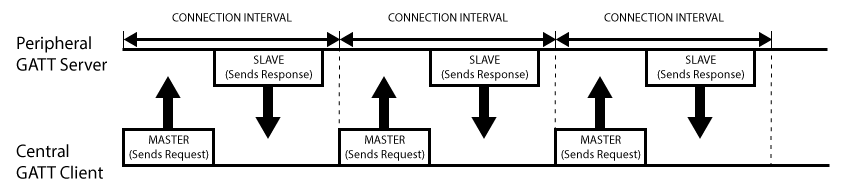
\includegraphics[width=0.9\textwidth]{gatt.png}
	\label{fig:gatt}
\end{figure}

\subsection{Profiles, Services and Characteristics}
As previously mentioned, GATT transactions make use of high-level nested objects called Profiles, Services and Characteristics.

\begin{itemize}
	\item Profile: it is the collection of Services on the device that has been compiled by the peripheral designers.
	
	\item Services: they contain specific chunks of data that are the Characteristics. A service can have one or more characteristics and each service is identified through a unique number called UUID, that can be either 16-bit or 128-bit depending on the manufacturing of the device. Services can be explored on the Services of the Bluetooth Developer Portal, thus it's easy to track a service and its purpose in case the Service is named "Unknown".
	
	\item Characteristics: this is the lowest level in a GATT transaction and contains a single data point (it may be a single value or an array of bytes, depending on the type of data transmitted). Characteristics are composed by various elements such as a type, a value, properties and permissions.
	Properties, in particular, define what another device can do with the characteristics over Bluetooth in terms of operations such as READ, WRITE or NOTIFY.
	\begin{itemize}
		\item READING a characteristic means copying the current value to the connected device.
		\item WRITING allows the connected device to insert new values of data.
		\item NOTIFICATIONS consist in a message type periodically sent in case of changes in a value.
	\end{itemize}
	Permissions specify the condition that must be met before reading or writing data to the characteristic is granted.
	
	\item Descriptors: there is another level below the Characteristics level, that contains meta-data related to it. For example it's possible enable or disable notifications through the Client Characteristic Configuration Descriptor.
\end{itemize}
